\documentclass [utf8] {article}
\usepackage{amsmath}
\usepackage{amsfonts}
\usepackage{amssymb}
\usepackage{geometry}
\usepackage{enumerate} 
\usepackage{graphicx}
\usepackage{indentfirst}
\usepackage{subcaption}
\usepackage{multirow}
\usepackage{float}
\usepackage{url}
\linespread{1.5}
\begin{document}
\begin{center}
\vspace*{2cm}
\rule{14cm}{0.5pt}\\
\Large{\textsc{UM-SJTU Joint Institute\\
Intro to Signals and Systems\\
(VE216)\\}}
\rule{14cm}{0.5pt}\\
\vspace*{3cm}
\Large{\textsc{Laboratory Report\\
Lab 1\\
LTI System}}
\vspace*{3cm}
\end{center}
\large{Name: Yiyang Xu\qquad ID:518370910020\\
Date: 9 June 2020}
\newpage

\section{Objectives}
{
    In this lab, we are going to learn:
    \begin{enumerate}
        \item Measuring the output response of the series RC circuit for a variety of inputs, including a step, a combination of a step and a ramp, and a sinusoid.
        \item Comparing results to those computed as part of pre-lab assignment.
    \end{enumerate}
}
\section{Theoretical Background}
{
    An RC circuit is used so that the computations are easy and physically meaningful. The same procedures can be applied to much more complicated systems.
\subsection{RC Circuit}
{
    The RC circuit shown below is an example of a simple LTI system. Of course, there are many other LTI systems that do not involve circuits at all.
    \begin{figure}[H]
        \begin{small}
            \begin{center}
                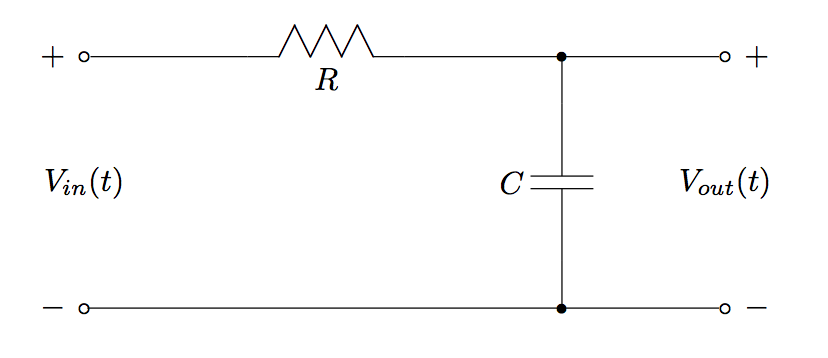
\includegraphics[width=0.95\textwidth]{figures/Figure1.png}
            \end{center}
            \caption{RC Circuit.}
            \label{fig:fig1}
        \end{small}
    \end{figure}

    We will take the system input to be the voltage $V_{in}(t)$, while the system output is the voltage, $V_{out}(t)$, dropped across the capacitor. Notice that these voltages, in general, will be functions of time, $t$.
}
\subsection{When Is A Linear Circuit A Linear System?}
{
    Using Kirchhoff's current and voltage laws, one can easily derive a differential equation model of the RC-circuit in Figure 1, namely
    \[R C \frac{d V_{o u t}(t)}{d t}+V_{o u t}(t)=V_{i n}(t) \tag{1}\]
    Appealing to basic knowledge of ODEs from a sophomore level math course, the total solution is seen to be
    \[V_{o u t}(t)=V_{0} e^{-t / R C}+\int_{0}^{t} \frac{1}{R C} e^{-(t-\tau) / R C} V_{i n}(\tau) d \tau, \quad t \geq 0 \tag{2}\]
    where the initial condition at time zero is $V_{out}(0) = V_0$. It is very easy to verify that $V_{out}(t)$ is a linear function $V_{in}(t)$ if, and only if, $V_{out}(0) = V_0 = 0$, that is, the initial voltage on the capacitor has to be zero. This point is emphasized because you will have to assure this in the laboratory by either waiting for the charge to decay on the capacitor or by shorting the capacitor with a wire.
}
\subsection{Impulse Response}
{
    The impulse response, $h(t)$, of an LTI system is, by definition, the output response when the input of the system is a delta function, $\delta(t)$. Of course, the delta function is a mathematical idealization. In practice, $h(t)$ can be well approximated by the response of the system when the input is a pulse of very short duration(compared with the response time of the system) and unit area, such as $p_{\Delta}(t)=\frac{1}{\Delta}(u(t)-u(t-\Delta))$ for $\Delta > 0 $ sufficiently small.
    \par Note that in order to keep the area of the pulse equal to unity, the amplitude has to increase as the pulse duration gets shorter. Often, this is a problem in a practical system as a large voltage pulse may fry an amplifier, for example. One way to get around this is to use linearity and realize that if the input is scaled by “$b$”, then the output will be scaled by “$b$” as well. Consequently, if the measured response is divided by “$b$”, an approximation of the impulse response is obtained
}
\subsection{Step Response}
{
    For any LTI system the output can be expressed as
    \[y(t)=x(t) * h(t)=\int_{-\infty}^{\infty} x(\tau) h(t-\tau) d \tau=\int_{-\infty}^{\infty} x(t-\tau) h(\tau) d \tau \tag{3}\]
    where $x(t)$ denotes the input and $*$ denotes the convolution operation. The output resulting when the input is a unit step function, $x(t) = u(t)$, is called the unit step response. Simple manipulation leads to
    \[y_{\text {step}}(t)=u(t) * h(t)=\int_{-\infty}^{\infty} h(\tau) u(t-\tau) d \tau=\int_{-\infty}^{t} h(\tau) u(t-\tau) d \tau+\int_{t}^{\infty} h(\tau) u(t-\tau) d \tau \tag{4}\]
    which, because the unit step function is equal to 1 for $t − \tau > 0$ and equal to 0 for $t − \tau < 0$ step response simplifies to
    \[y_{\text {step}}(t)=\int_{-\infty}^{t} h(\tau) d \tau \tag{5}\]
    By taking the derivative of $y_{step}(t)$ with respect to $t$, we obtain, by the fundamental theorem of calculus,
    \[\frac{d y_{s t e p}(t)}{d t}=\frac{d}{d t} \int_{-\infty}^{t} h(\tau) d \tau=h(t) \tag{6}\]
    Thus the impulse response can be computed from the unit step response by calculating the derivative of the step response with respect to time. This is a useful observation because it is sometimes easier to apply a step input to a physical system than it is to apply (an approximation of) an impulse.
}
}

\section{Experiment Procedures}{
    \subsection{Step Response}{
        \begin{enumerate}
            \item I first drew the circuit via Proteus.
            \item I adjust the scale to the most suitable range.
            \item I ran the simulation and record the result.
        \end{enumerate} 
    }
    \subsection{Pulse Response}{
        \begin{enumerate}
            \item I change the input to a pulse response and keeps the rest of the circuit the same.
            \item I repeated the procedure in the first part.
        \end{enumerate}
    }
    \subsection{Ramp Response}{
        \begin{enumerate}
            \item I change the input to a ramp response and repeated the procedure in the previous sections.
        \end{enumerate}
    }
    \subsection{Sine Response}{
        \begin{enumerate}
            \item I change the input to a sine response and repeat the same procedure.
        \end{enumerate}
    }
}

\section{Experimental Results}
{
    \subsection{Step Response}
    {
        \begin{figure}
            \begin{small}
                \begin{center}
                    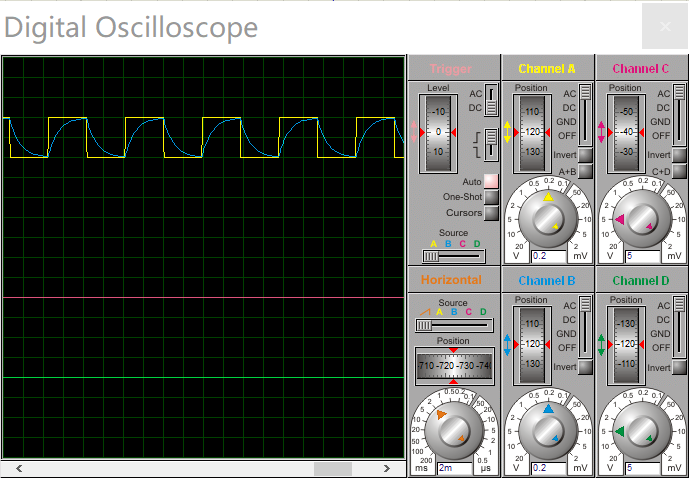
\includegraphics[width=0.6\textwidth]{figures/Figure2.png}
                \end{center}
                \caption{Step Response Simulation}
                \label{fig:fig2}
            \end{small}
        \end{figure}
        The graph shows the step response in this lab experimentally. Comparing to the plot we get in pre-lab1, the result is similar in each period which is shown in the following figure.

        \begin{figure}[H]
            \begin{small}
                \begin{center}
                    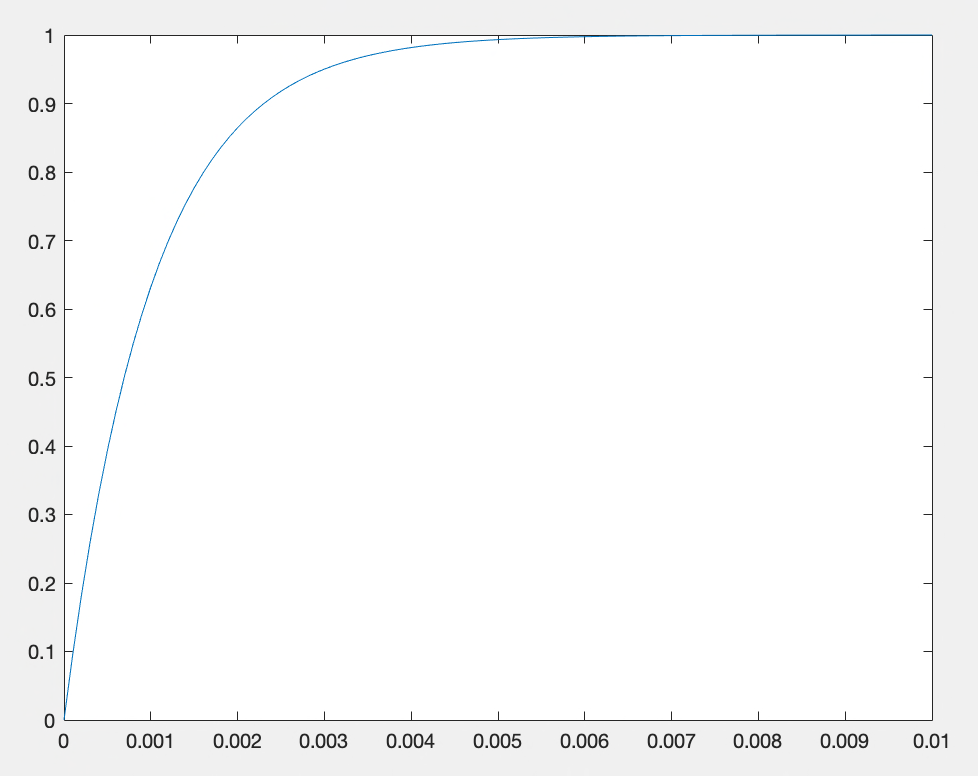
\includegraphics[width=0.6\textwidth]{figures/Figure2_1.png}
                \end{center}
                \caption{Theoretical Step Response in One Period}
                \label{fig:fig2_1}
            \end{small}
        \end{figure}
    }

    \subsection{Pulse Response}
    {
        The following figure gives the pulse response whose pulse has a width of $1ms$ and amplitude of $100mV$.

        \begin{figure}[H]
            \begin{small}
                \begin{center}
                    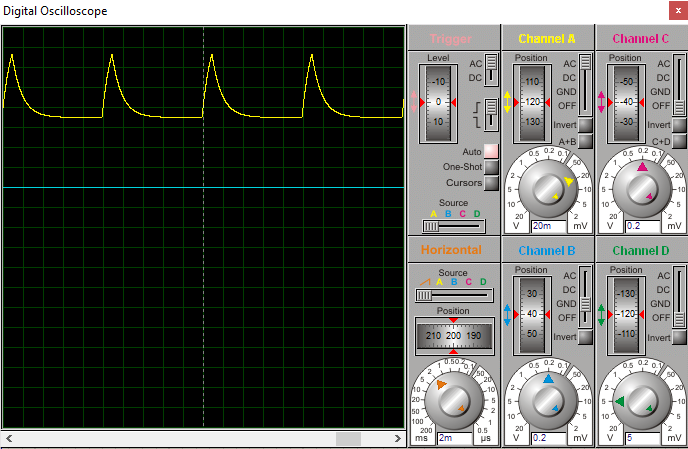
\includegraphics[width=0.6\textwidth]{figures/Figure3.png}
                \end{center}
                \caption{Pulse Response Simulation (Width = $1ms$, Amplitude = $100mV$)}
                \label{fig:fig3}
            \end{small}
        \end{figure}

        By comparison, we switch to the width of $0.5ms$ and amplitude of $200mV$ and simulate again to obtain a figure with slightly difference in scale.

        \begin{figure}[H]
            \begin{small}
                \begin{center}
                    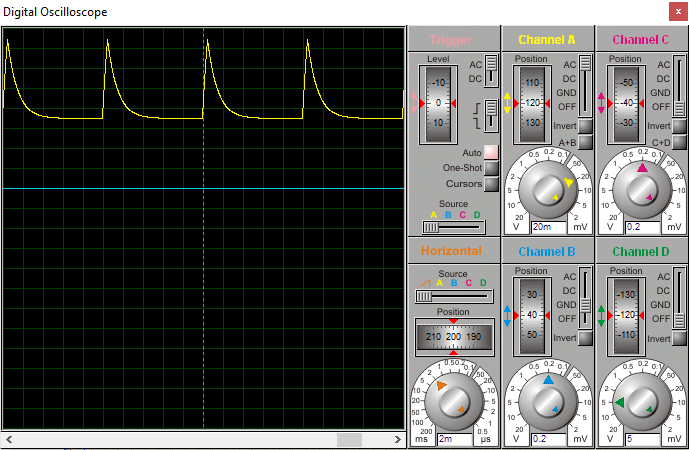
\includegraphics[width=0.6\textwidth]{figures/Figure4.png}
                \end{center}
                \caption{Pulse Response Simulation (Width = $1ms$, Amplitude = $100mV$)}
                \label{fig:fig4}
            \end{small}
        \end{figure}
    
    }

    \subsection{Ramp Response}
    {
        The graph shows the ramp response. The yellow line represents the input signal while the blue line is the output.
        \begin{figure}[H]
            \begin{small}
                \begin{center}
                    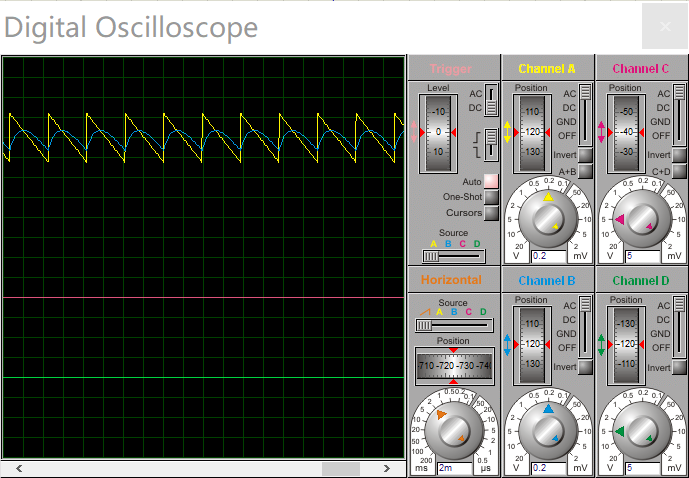
\includegraphics[width=0.6\textwidth]{figures/Figure5.png}
                \end{center}
                \caption{Ramp Response Simulation}
                \label{fig:fig4}
            \end{small}
        \end{figure}
        
    }

    \subsection{Sine Response}
    {
        In this part, we switch the input channel as $50Hz$, $500Hz$ and $5kHz$ as is shown in the following figures. By observation, we are able to make the table to record the Frequency, $V_{out}$ / $V_{in}$, Time Shift and Phase Shift.
        \begin{figure}[H]
            \begin{small}
                \begin{center}
                    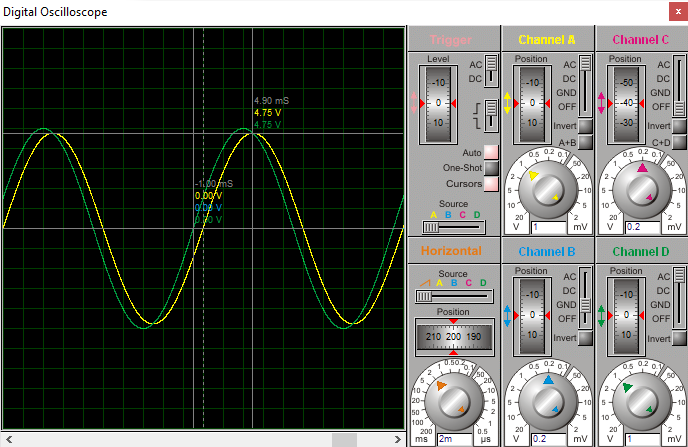
\includegraphics[width=0.5\textwidth]{figures/Figure6.png}
                \end{center}
                \caption{Sine Response Simulation ($f = 50Hz$)}
                \label{fig:fig5}
            \end{small}
        \end{figure}

        \begin{figure}[H]
            \begin{small}
                \begin{center}
                    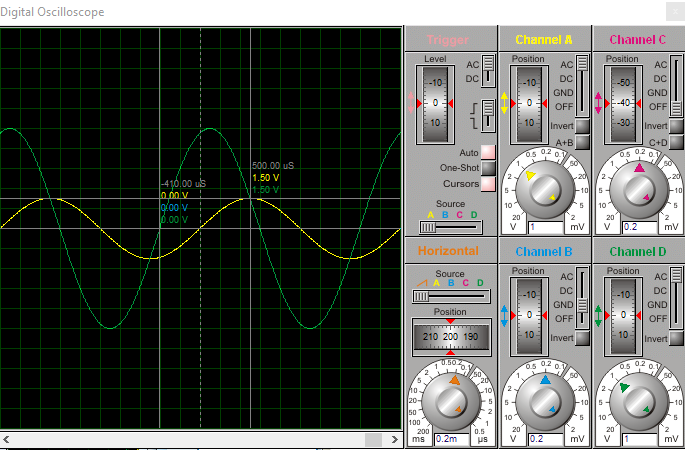
\includegraphics[width=0.5\textwidth]{figures/Figure7.png}
                \end{center}
                \caption{Sine Response Simulation ($f = 500Hz$)}
                \label{fig:fig6}
            \end{small}
        \end{figure}

        \begin{figure}[H]
            \begin{small}
                \begin{center}
                    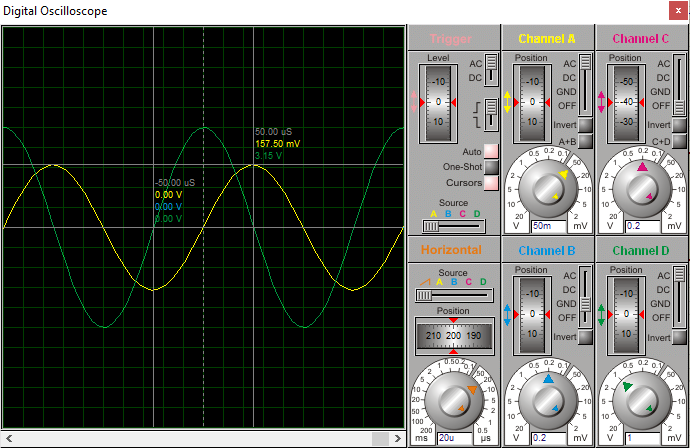
\includegraphics[width=0.5\textwidth]{figures/Figure8.png}
                \end{center}
                \caption{Sine Response Simulation ($f = 5kHz$)}
                \label{fig:fig7}
            \end{small}
        \end{figure}
        
        \begin{table}[h]
            \centering
            \begin{tabular}{|c|c|c|c|}
                \hline
                Frequency (Hz) & $V_{out}$ / $V_{in}$ & Time Shift & Phase Shift \\
                \hline
                50      &    0.950   &    $1.00ms$        & $-18.0^{\circ}$\\
                500     &    0.300  &    $0.410ms$        & $-72.8^{\circ}$\\
                5000    &    0.00320    &   $0.0510ms$         &    $-90.0^{\circ}$\\
                \hline            
            \end{tabular}
            \caption{Sine Response Simulation Results}
            \label{table:tb1}
        \end{table}

        According to what we have learnt in the pre-lab, we can calculate the phase shift via the equation $\theta = -ft$. 


        Therefore, we can compare it with the theoretical value which is listed in the following table.

        \begin{table}[h]
            \centering
            \begin{tabular}{|c|c|c|c|}
                \hline
                Frequency (Hz) & $V_{out}$ / $V_{in}$ & Time Shift & Phase Shift \\
                \hline
                50      &    0.9540   &    $0.9689ms$        & $-17.4406^{\circ}$\\
                500     &    0.3033  &    $0.4019ms$        & $-72.3432^{\circ}$\\
                5000    &    0.00318    &   $0.04899ms$         &    $-88.1768^{\circ}$\\
                \hline            
            \end{tabular}
            \caption{Sine Response Theoretical Results}
            \label{table:tb1}
        \end{table}  
    }
}

\section{Discussion and Conclusion}
{
    \begin{enumerate}
        \item In the Step Response Simulation, we see that the theoretical curve of step response is close to the experimental curve in each period. Therefore, we've verified the pulse response can be expressed as $y(t) = (1-e^{-\frac{t}{RC}})u(t)$
        \item In the Pulse Response Simulation, the simulation result also meets our expectation. Therefore, we've verified that the step response can be expressed as $y(t) = \frac{1}{RC}e^{-\frac{t}{RC}}$
        \item In the Ramp Response Simulation, we've learned that the ramp response here can be considered as a sum of the step response and the time integral of the step response.
        \item In the Sine Response, by comparing with the experimental and theoretical value of the Frequency, $V_{out}$ / $V_{in}$, Time Shift and Phase Shift. The result are close which indicate our experiment is successful.
    \end{enumerate}
}
\newpage
\begin{thebibliography}{99}
    \bibitem{r1} VE 216, "Spring 2020 Lab 1: LTI Systems Part I: Intro \& Pre-lab Assignment," Accessed on: Jun. 8, 2020. [Online]. Available: \url{https://umjicanvas.com/courses/1527/files/folder/Lab}.
\end{thebibliography}

\end{document}